%
% $RCSfile: models.tex,v $
%
% Copyright (C) 2002-2008. Christian Heller.
%
% Permission is granted to copy, distribute and/or modify this document
% under the terms of the GNU Free Documentation License, Version 1.1 or
% any later version published by the Free Software Foundation; with no
% Invariant Sections, with no Front-Cover Texts and with no Back-Cover
% Texts. A copy of the license is included in the section entitled
% "GNU Free Documentation License".
%
% http://www.cybop.net
% - Cybernetics Oriented Programming -
%
% http://www.resmedicinae.org
% - Information in Medicine -
%
% Version: $Revision: 1.1 $ $Date: 2008-08-19 20:41:07 $ $Author: christian $
% Authors: Christian Heller <christian.heller@tuxtax.de>
%

\subsubsection{Models}
\label{models_heading}
\index{Communication Models}
\index{Agent as Social System}
\index{Communication Model by Shannon \& Weaver}
\index{Conversation Model by Osgood \& Schramm}
\index{Encoder}
\index{Decoder}
\index{Contents of Communication}
\index{Lasswell Formula}
\index{Sender (Who) as Communication Element}
\index{Receiver (Whom) as Communication Element}
\index{Message (What) as Communication Element}
\index{Language (Channel) as Communication Element}
\index{Result (Effect) as Communication Element}

Section \ref{agent_oriented_programming_heading} described a (software)
\emph{Agent} as \emph{social} system communicating with other agents, including
human beings \cite[p. 330]{sowa}. Various communication process models were
contributed by the \emph{Social Sciences}. Buesch \cite{buesch} describes a
\emph{Mathematical Communication Model} by Shannon \& Weaver (figure
\ref{shannon_figure}) that shows very well the presence of two translators:
\emph{Encoder} and \emph{Decoder}.

\begin{figure}[ht]
    \begin{center}
        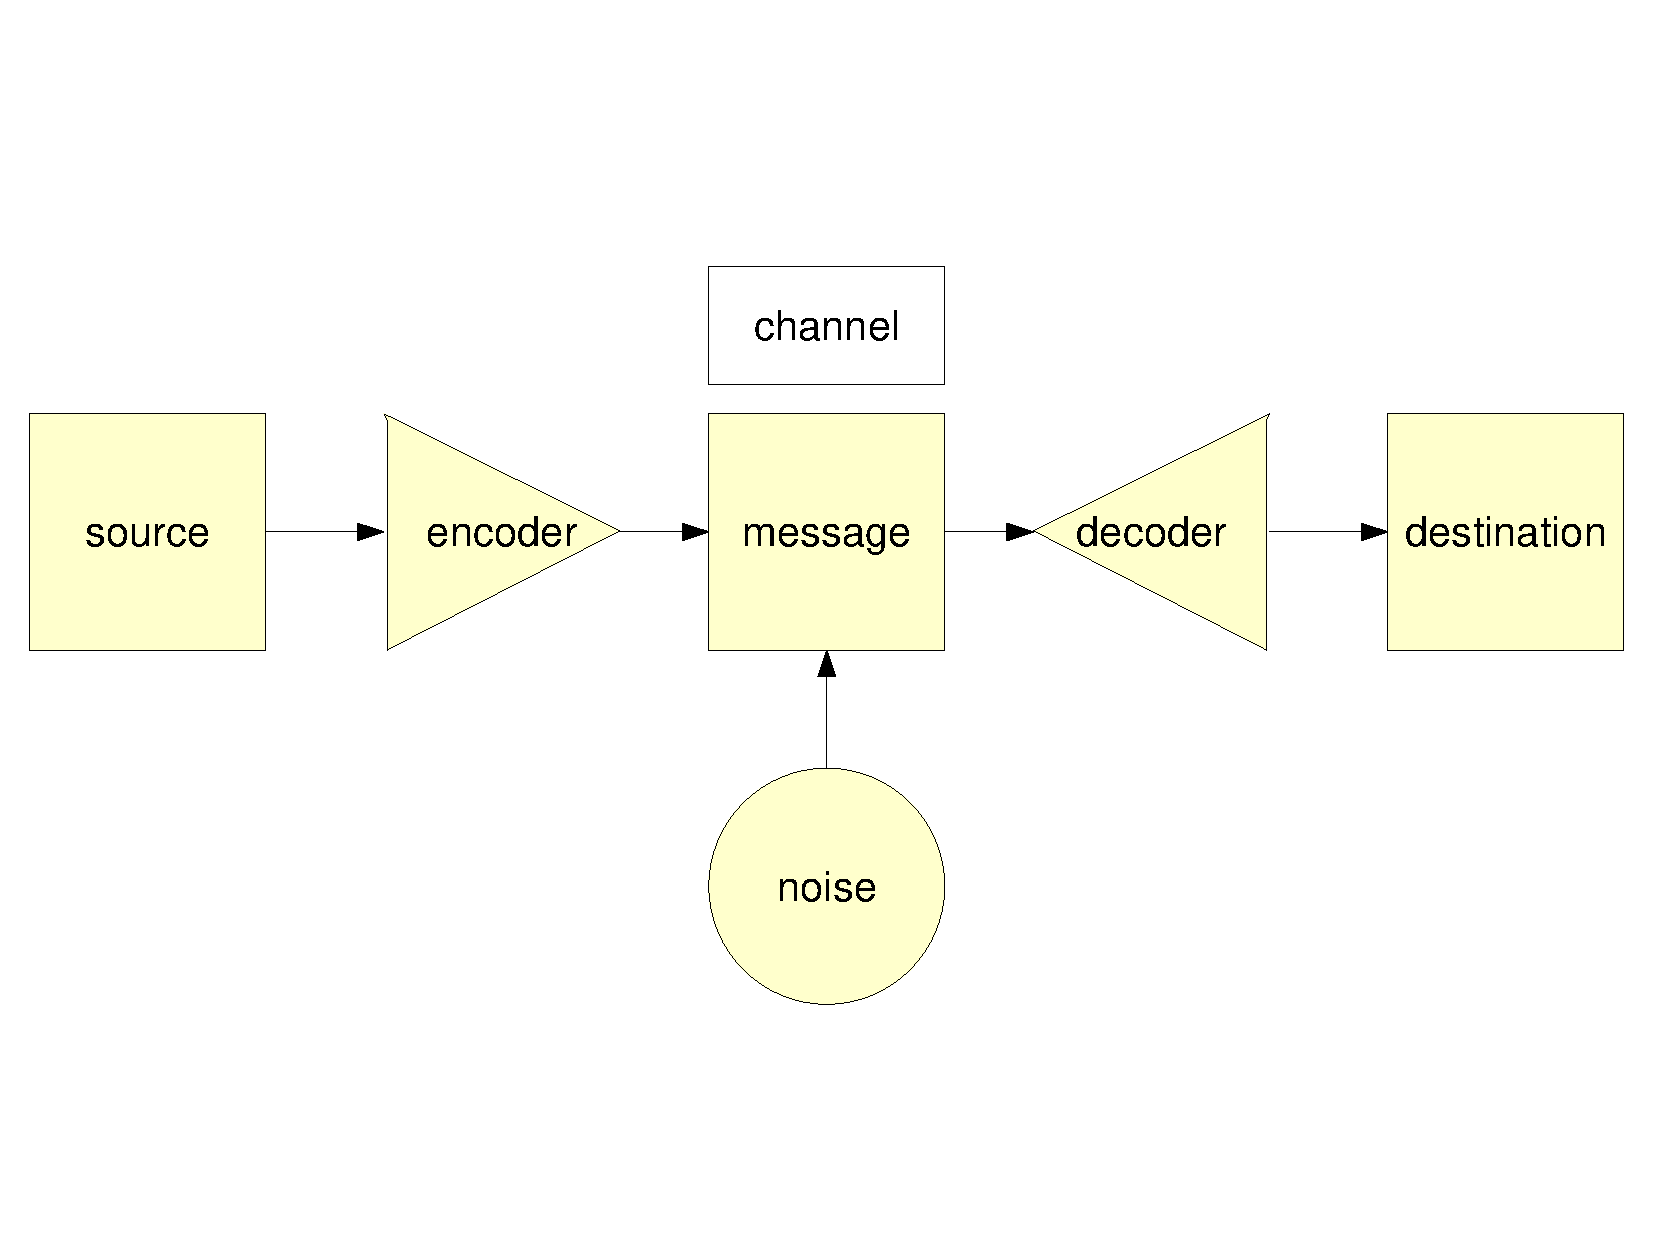
\includegraphics[scale=0.3,angle=-90]{graphic/shannon.pdf}
        \caption{Mathematical Communication Model by Shannon \& Weaver \cite{shannon}}
        \label{shannon_figure}
    \end{center}
\end{figure}

The \emph{Conversation Model} of Osgood \& Schramm (figure \ref{osgood_figure})
extends the communication model to a circular process of \emph{Question} and
\emph{Answer}, of \emph{Sending} and \emph{Receiving}. It shows more clearly,
that \emph{every} system, in order to communicate both ways, needs to own an
\emph{encoding} as well as a \emph{decoding} translator. The interpreter system
introduced in chapter \ref{cybernetics_oriented_interpreter_heading} contains
both kinds of translators.

\begin{figure}[ht]
    \begin{center}
        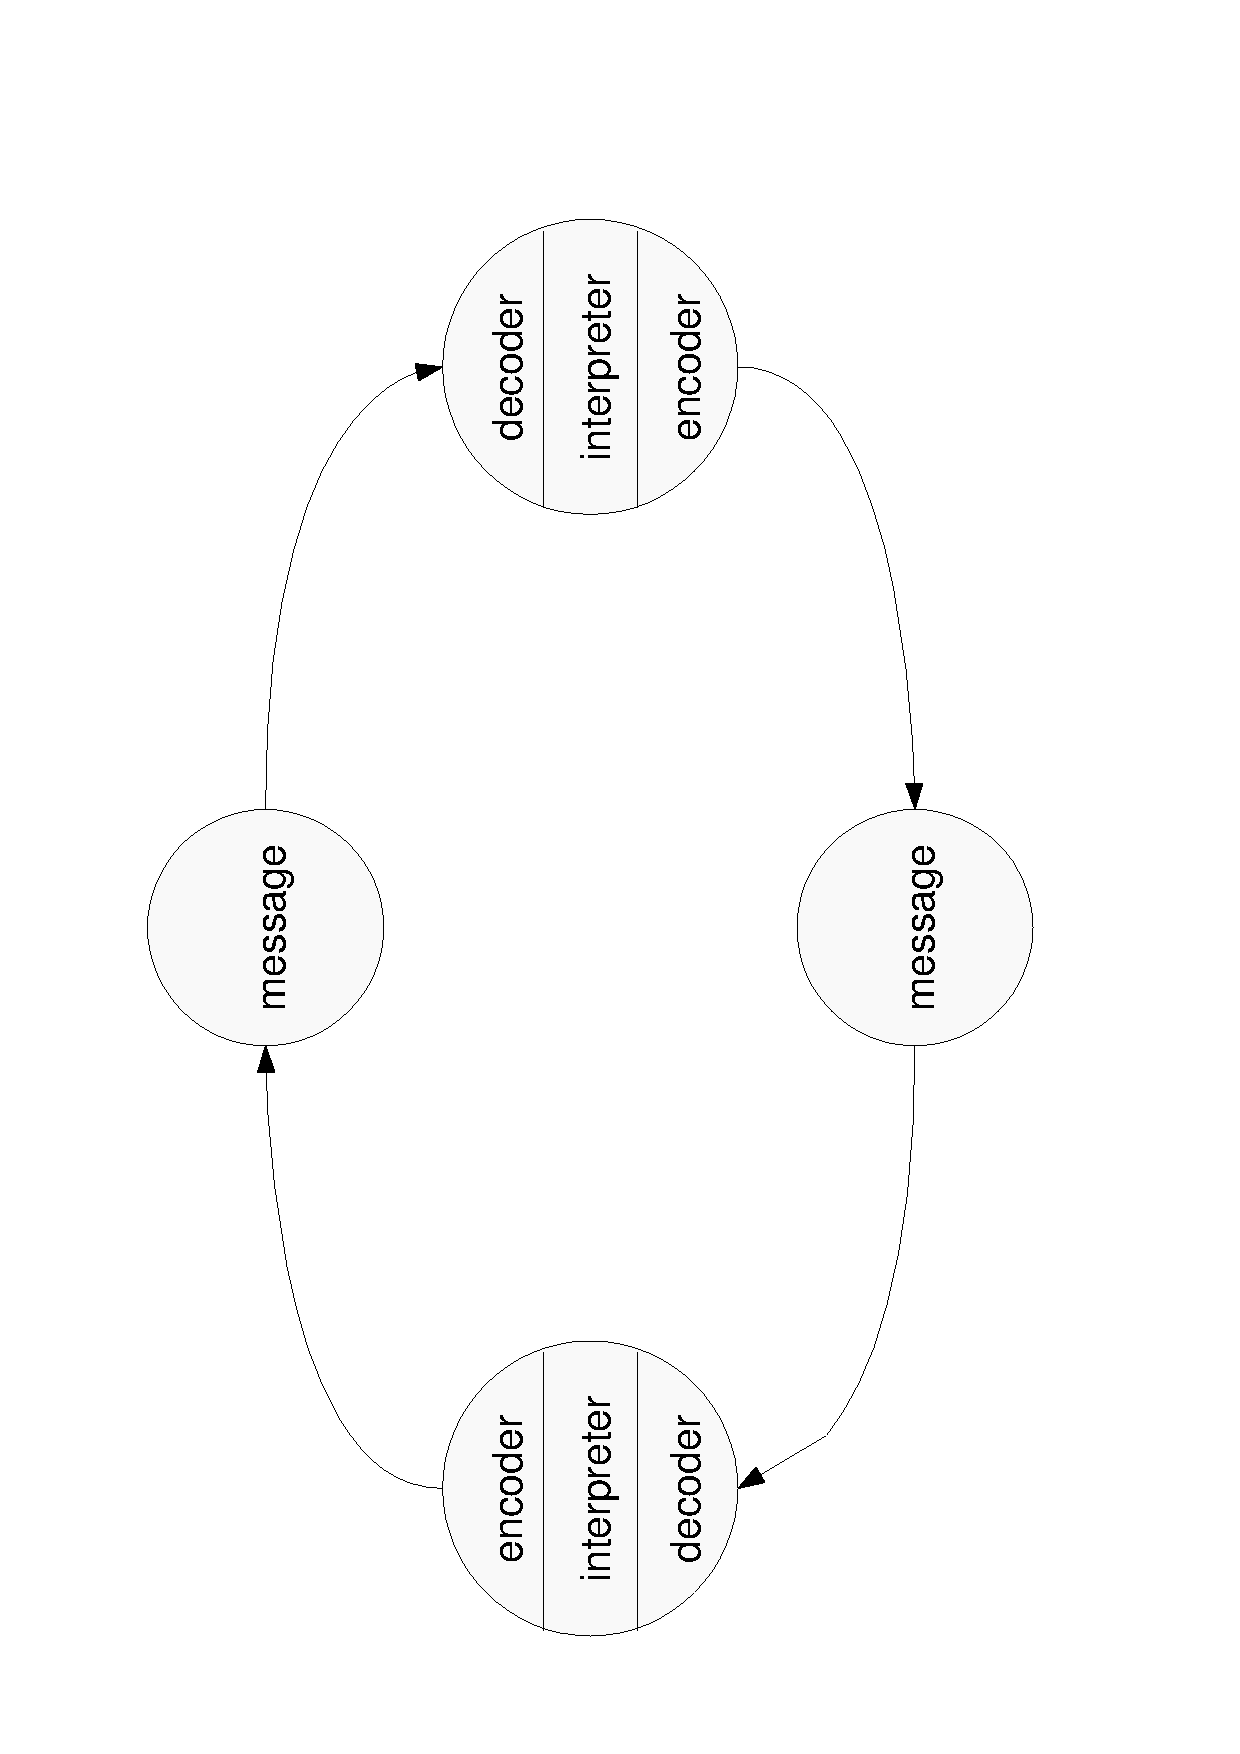
\includegraphics[scale=0.3,angle=-90]{graphic/osgood.pdf}
        \caption{Conversation Model by Osgood \& Schramm \cite{osgood}}
        \label{osgood_figure}
    \end{center}
\end{figure}

The \emph{Contents of Communication} is described by the
\emph{Lasswell Formula} (figure \ref{lasswell_figure}). After it, communication
consists of the five elements: \emph{Sender} (Who) and \emph{Receiver} (Whom),
\emph{Message} (What), \emph{Language} (Channel) and \emph{Result} (Effect).
The first four of these will be considered in the specification of the
knowledge modelling language introduced in chapter
\ref{cybernetics_oriented_language_heading}. The effects a communication has
(fifth element) are not a prerequisite for that communication to happen and
thus not interesting in the context of its technical realisation, as
investigated later in this work.

\begin{figure}[ht]
    \begin{center}
        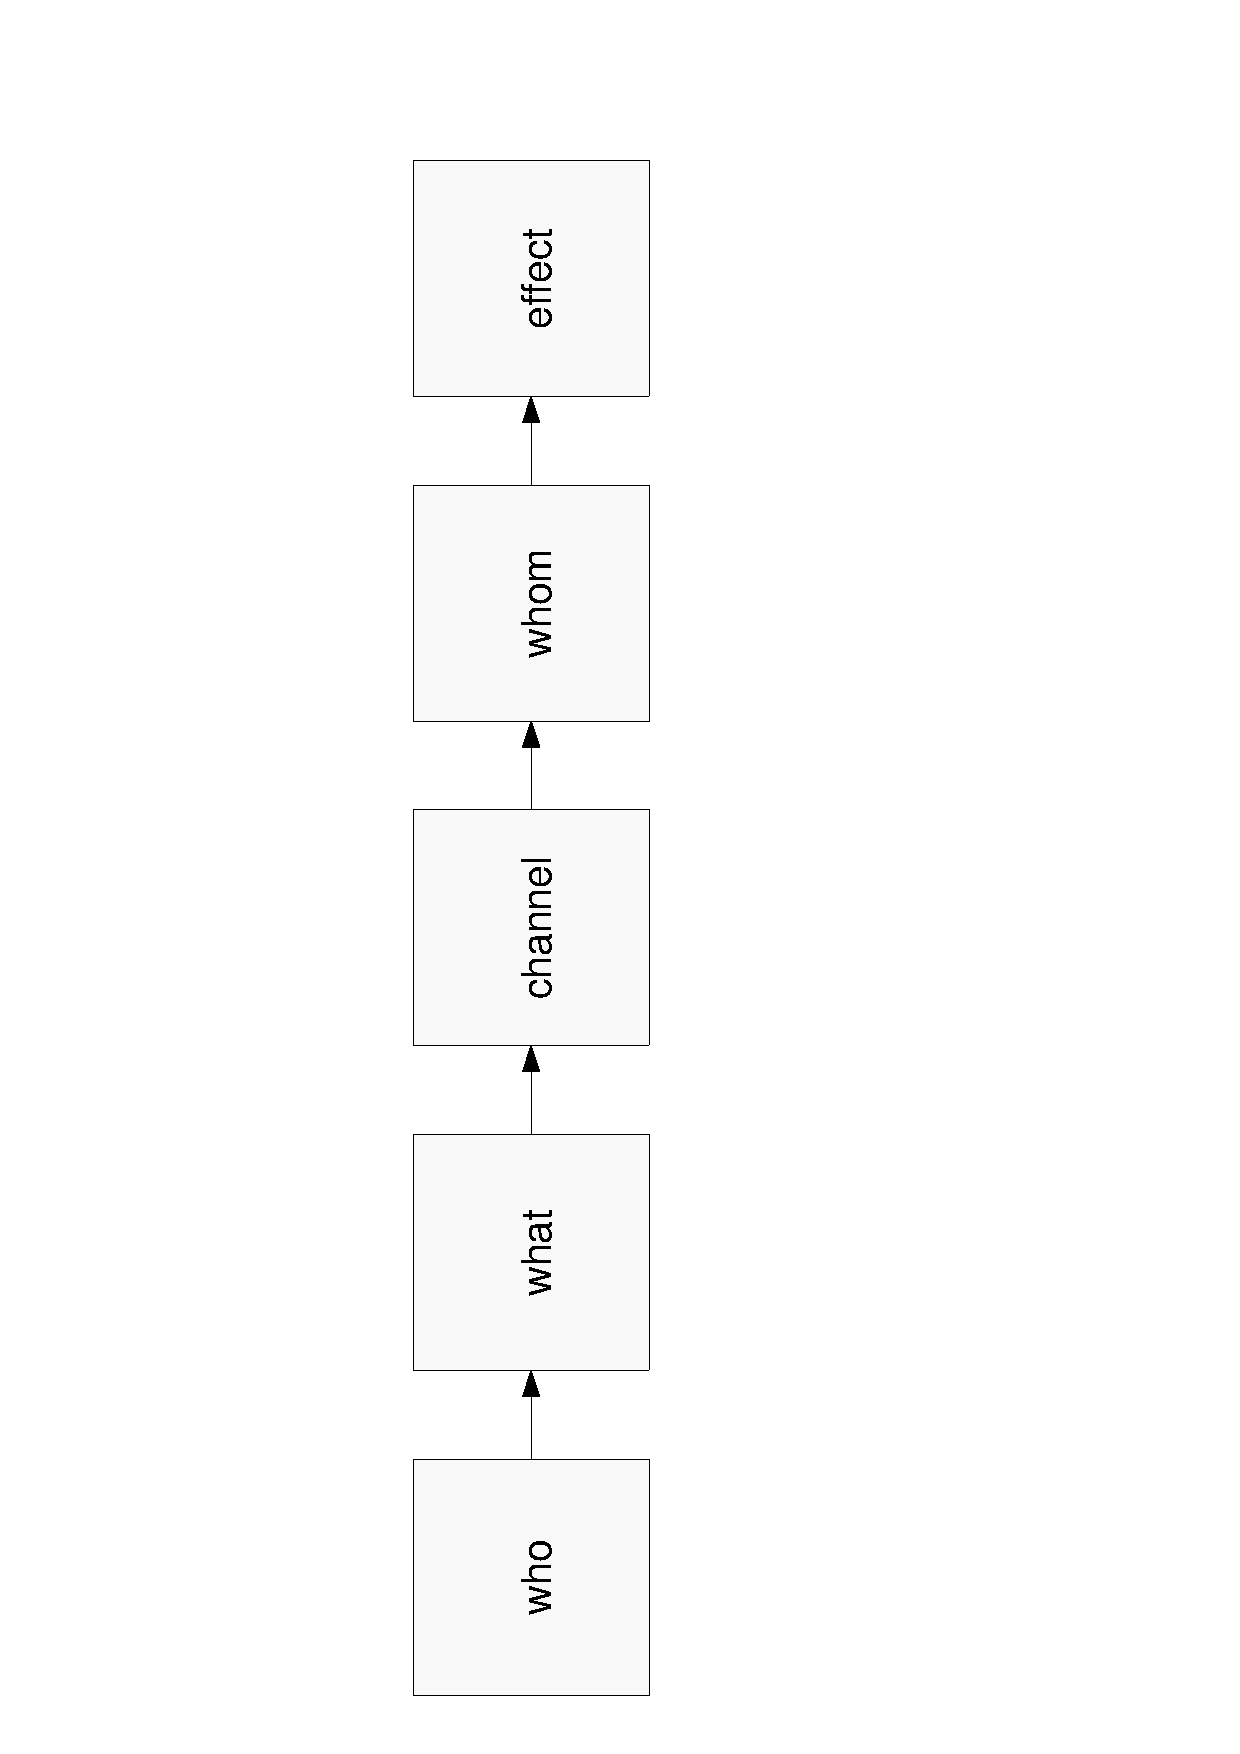
\includegraphics[scale=0.3,angle=-90]{graphic/lasswell.pdf}
        \caption{Contents of Communication (Lasswell Formula) \cite{lasswell}}
        \label{lasswell_figure}
    \end{center}
\end{figure}
